\frame{
  \frametitle{Introduction}

  \begin{itemize}
    \item Billiard ball bouncing in a square
    \item Assume no gravity or friction
  \end{itemize}
}

\subsection{Basic Notation}

\frame{
  \frametitle{Basic Notation}
  \begin{definition}
    A table $T \subset \R^2$ is the unit square. Vertical sides are labelled with a $v$. Horizontal sides are labelled with an $h$.
  \end{definition}

  \begin{figure}
    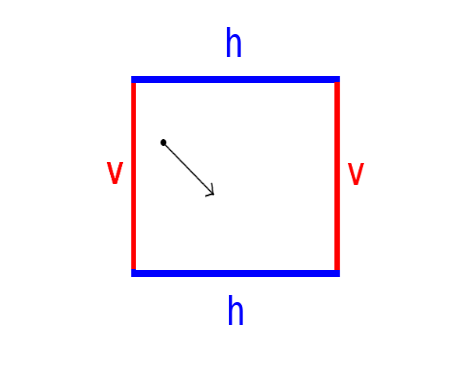
\includegraphics[width=2in]{square_with_sides.png}
  \end{figure}
}

\frame{
  \frametitle{Notation}

  \begin{definition}
     A ball $p \in T$ begins at position $\vec{r}_0 \in T$ with initial velocity $\vec{v}_0 \ne 0$. When the ball collides with an edge of the table, it reflects its angle with the table edge.
  \end{definition}

  \begin{figure}
    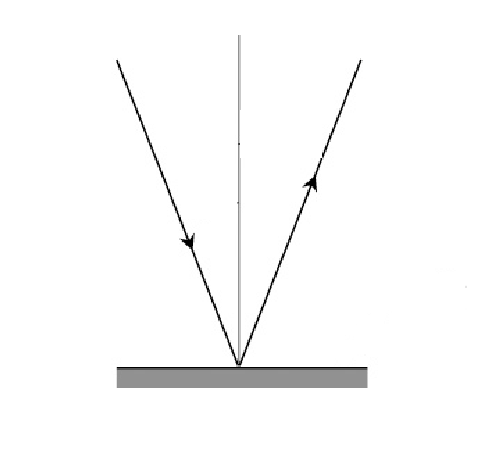
\includegraphics[height=1.5in]{particle_collision.png}
  \end{figure}
}

\subsection{Examples}

\frame{
  \frametitle{Example}

  \begin{example}
    Examine the periodic sequence: `abab`
  \end{example}

  \begin{figure}
    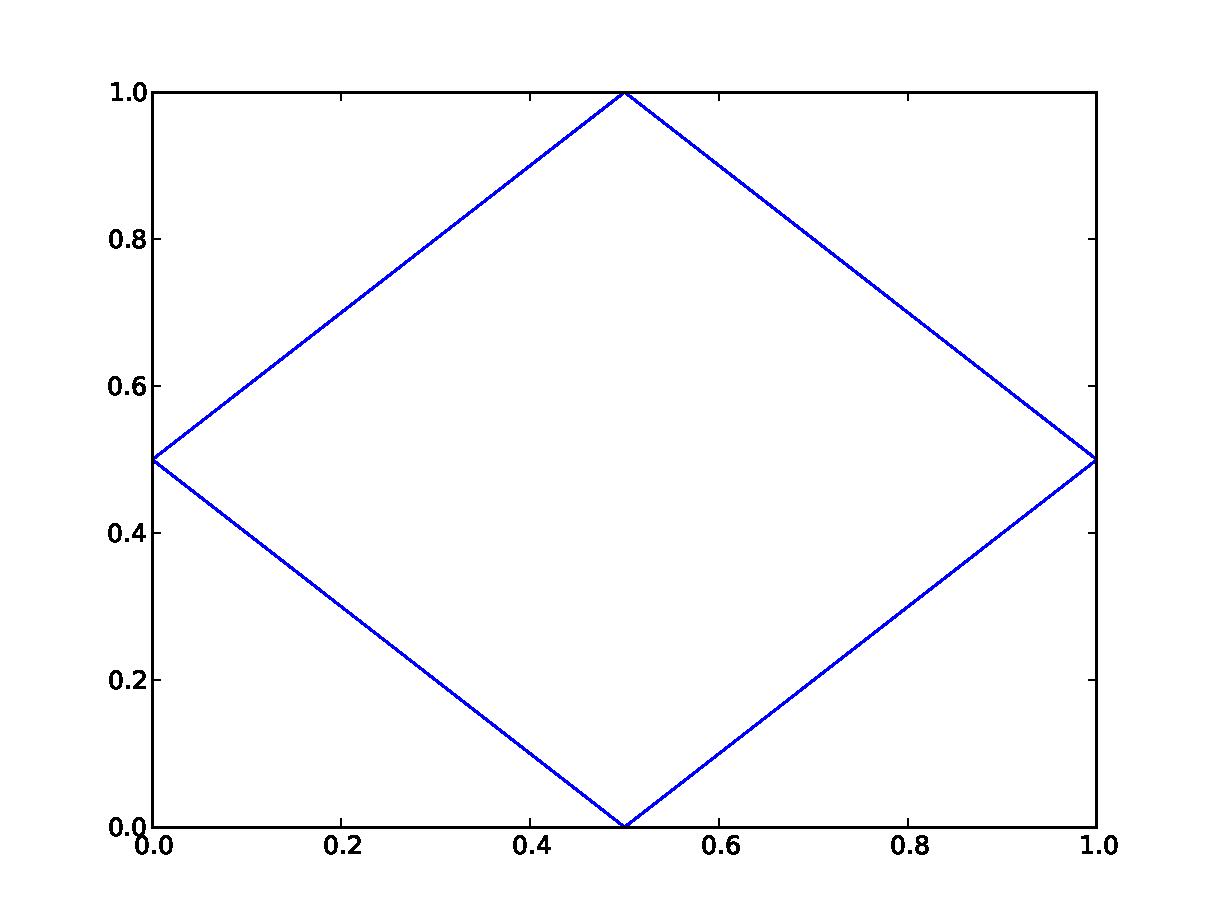
\includegraphics[width=3in]{abab.pdf}
  \end{figure}
}

\frame{
  \frametitle{Another Example}

  \begin{example}
    Examine the periodic sequence: `aaabaaab`
  \end{example}

  \begin{figure}
    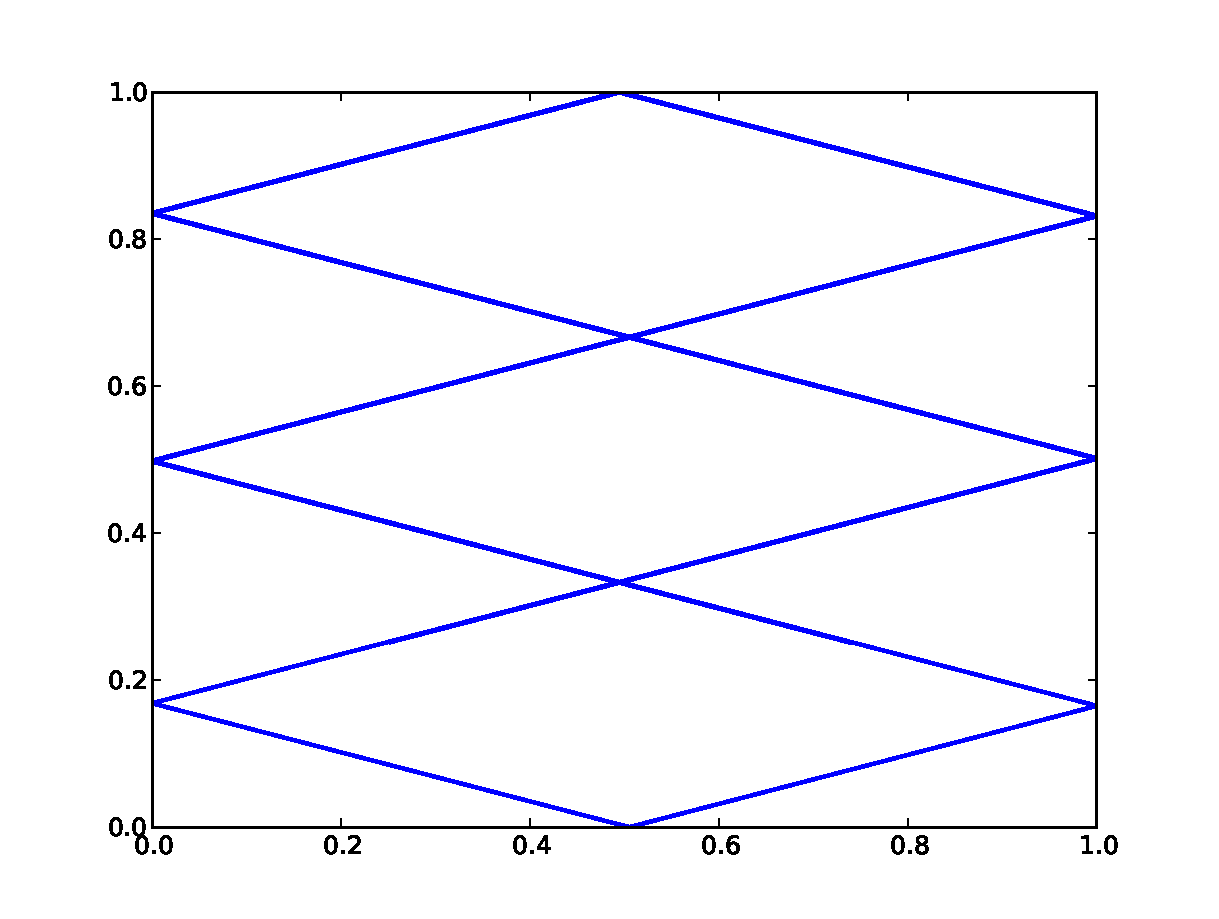
\includegraphics[width=3in]{aaabaaab.pdf}
  \end{figure}
}

\subsection{Problem Statement}

\frame{
  \frametitle{Problem Statement}

  Problem: Characterize the properties of collision sequences.

  \begin{itemize}
    \item Given a sequence of $a$'s and $b$'s, determine if it is a valid collision sequence.
    \item Given a valid collision sequence, determine a possible starting position and velocity.
  \end{itemize}
}

\subsection{Outline}

\frame{
  \frametitle{Presentation Outline}
  \tableofcontents
}


\subsection{Primary and Secondary Sides}

\frame{
  \frametitle{Secondary Side Theorem}

  \begin{theorem}
    At least one side will never have more than one consecutive occurrence in a valid collision string.
  \end{theorem}
}

\frame{
  \frametitle{Secondary Side Theorem Examples}

  \begin{example}
    Valid: $vhhhvhhhv$
  \end{example}

  \begin{example}
    Valid: $vhvhvhv$
  \end{example}

  \begin{example}
    Valid: $vvvvvhvvvvhvvvvvhvvvv$
  \end{example}

  \begin{example}
    Invalid: $vvhhhvvvhhhvvhhh$
  \end{example}

  \begin{example}
    Invalid: $vhhhvvhvh$
  \end{example}
}

\frame{
  \frametitle{Secondary Side Theorem Proof}

  \begin{itemize}
    \item A billiard ball trajectory must be a line in the tiled grid with slope $m$.
    \item Case 1: $m = 1$.
    \item Case 2: $m < 1$ or $m > 1$.
  \end{itemize}
}

\frame{
  \frametitle{Secondary Side Theorem Proof}

  If $m = 1$, $v$ and $h$ alternate.

  % TODO: show a picture here
}

\frame{
  \frametitle{Secondary Side Theorem Proof}

  If $m < 1$, there must exist an $h$ between each $v$.

  If $m > 1$, similar argument holds.

  % TODO: show a picture of a single square in the lattice, 
}

\frame{
  \frametitle{Notation}
  \begin{definition}
    \textbf{Secondary side}: a side which never has more than one consecutive occurrences.
    \textbf{Primary side}: a side which is not a secondary side.
  \end{definition}

  \pause

  \begin{definition}
    \textbf{Primary substring:} a subsequence from the collision string which contains a consecutive sequence of primary sides.
  \end{definition}

  \pause

  \begin{example}
    \textbf{Collision string}: $vvhvvvhvvhvvvh$
    \textbf{Secondary Side}: $h$
    \textbf{Primary Side}: $v$
    \textbf{Primary substrings}: $vv$, $vvv$
  \end{example}
}

